\documentclass[tikz,border=5pt]{standalone}
\usepackage{tikz}
\usetikzlibrary{arrows.meta, positioning, decorations.text, calc}

\begin{document}

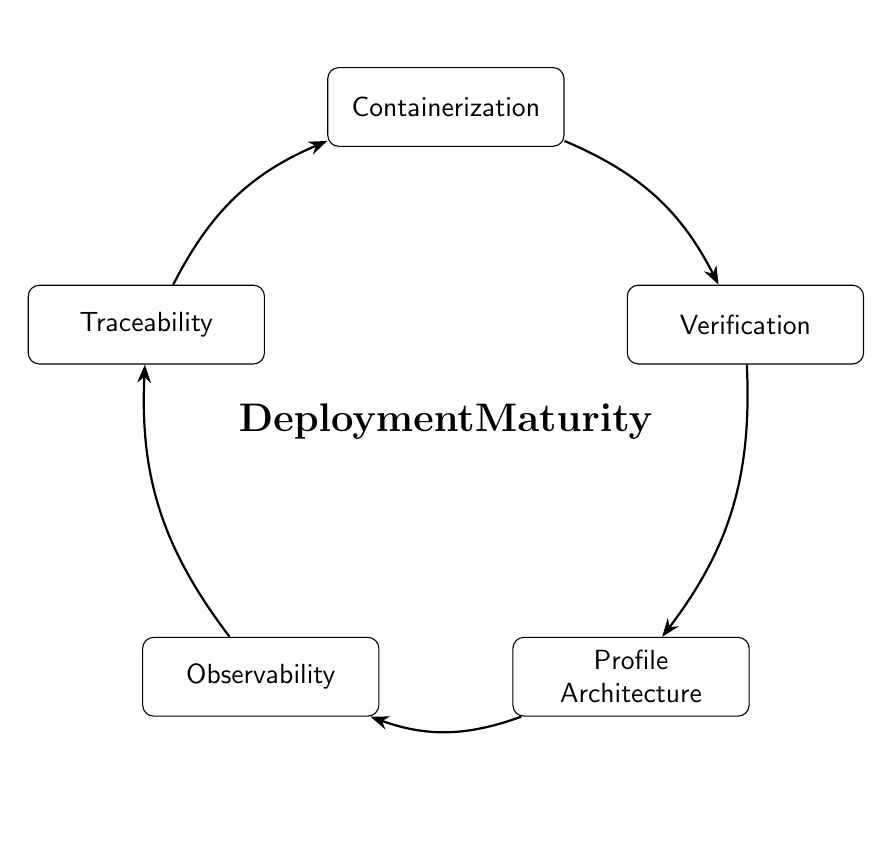
\begin{tikzpicture}[
    node style/.style={
        draw,
        rounded corners,
        minimum width=3cm,
        minimum height=1cm,
        align=center,
        font=\sffamily
    },
    arrow style/.style={
        thick,
        ->,
        >=Stealth
    }
]

% Radius
\def\radius{4}

% Nodes on circumference
\node[node style] (C) at (90:\radius)  {Containerization};
\node[node style] (V) at (18:\radius)  {Verification};
\node[node style] (P) at (-54:\radius) {Profile\\Architecture};
\node[node style] (O) at (-126:\radius){Observability};
\node[node style] (T) at (162:\radius) {Traceability};

% Curved arrows (cycle)
\draw[arrow style] (C) to[bend left=20] (V);
\draw[arrow style] (V) to[bend left=20] (P);
\draw[arrow style] (P) to[bend left=20] (O);
\draw[arrow style] (O) to[bend left=20] (T);
\draw[arrow style] (T) to[bend left=20] (C);

% Optional central label
\node at (0,0) {\Large\textbf{Deployment\\Maturity}};

% Optional curved text annotation (example)
\draw[
    decorate,
    decoration={
        text along path,
        text align=center,
        text={|\small\sffamily|
            } }
] (90:\radius+1) arc (90:-270:\radius+1);

\end{tikzpicture}

\end{document}
